\documentclass[12pt, a4paper]{article}

% ─── Packages ───────────────────────────────────────────────────────────────
\usepackage[utf8]{inputenc}
\usepackage[T1]{fontenc}
\usepackage{lmodern}
\usepackage[margin=1in]{geometry}
\usepackage{graphicx}
\usepackage{float}
\usepackage{hyperref}
\usepackage{booktabs}
\usepackage{enumitem}
\usepackage{xcolor}
\usepackage{titlesec}
\usepackage{fancyhdr}
\usepackage{caption}
\usepackage{subcaption}
\usepackage{longtable}
\usepackage{array}
\usepackage{parskip}
\usepackage{setspace}

% ─── Colours ────────────────────────────────────────────────────────────────
\definecolor{brand}{HTML}{6366F1}
\definecolor{darkbg}{HTML}{1E1B4B}
\definecolor{success}{HTML}{10B981}
\definecolor{warning}{HTML}{F59E0B}

% ─── Header / Footer ───────────────────────────────────────────────────────
\pagestyle{fancy}
\fancyhf{}
\fancyhead[L]{\small\textcolor{brand}{EduSubmit — HCI Design Report}}
\fancyhead[R]{\small\thepage}
\renewcommand{\headrulewidth}{0.4pt}

% ─── Section styling ───────────────────────────────────────────────────────
\titleformat{\section}{\Large\bfseries\color{darkbg}}{\thesection}{1em}{}[\vspace{-0.5em}\rule{\textwidth}{0.4pt}]
\titleformat{\subsection}{\large\bfseries\color{brand}}{\thesubsection}{1em}{}

\hypersetup{
  colorlinks=true,
  linkcolor=brand,
  urlcolor=brand,
  citecolor=brand
}

\graphicspath{{images/}}

% ═══════════════════════════════════════════════════════════════════════════
\begin{document}

% ─── Title Page ─────────────────────────────────────────────────────────────
\begin{titlepage}
\centering
\vspace*{2cm}
{\Huge\bfseries\textcolor{darkbg}{HCI-Driven Design Report}\\[0.4cm]}
{\LARGE\textcolor{brand}{EduSubmit: Assignment Submission System}\\[1.5cm]}
\rule{\textwidth}{1pt}\\[1cm]
{\Large\textbf{Course:} Human-Computer Interaction}\\[0.3cm]
{\Large\textbf{Submitted by:} [Student Name]}\\[0.3cm]
{\Large\textbf{Student ID:} [Your ID]}\\[0.3cm]
{\Large\textbf{Date:} February 26, 2026}\\[1cm]
\rule{\textwidth}{1pt}\\[2cm]

\textit{This report documents the process-driven design of a Learning Management Assignment Submission System, applying HCI principles, usability heuristics, and iterative evaluation throughout every phase of development.}

\vfill
{\small Department of Computer Science\\University Name}
\end{titlepage}

% ─── Table of Contents ─────────────────────────────────────────────────────
\tableofcontents
\newpage

% ═══════════════════════════════════════════════════════════════════════════
\section{Introduction}

In this project, I designed and developed \textbf{EduSubmit}—a web-based assignment submission system—following a structured Human-Computer Interaction (HCI) methodology. Rather than focusing purely on aesthetics, I treated the interface as a research-backed product grounded in real usability problems, validated through HCI theories, and iteratively refined through simulated usability testing.

The motivation came from well-known frustrations in existing Learning Management Systems (LMS):
\begin{itemize}[noitemsep]
  \item Confusing or ambiguous submission deadlines
  \item File upload failures with no explanation
  \item No clear confirmation after submission
  \item Poor visibility of grades and instructor feedback
  \item Overloaded dashboards causing cognitive overload
  \item Accessibility barriers for keyboard-only and screen-reader users
\end{itemize}

My goal was to address each of these problems using specific, traceable HCI principles—not guesswork.

% ═══════════════════════════════════════════════════════════════════════════
\section{Problem Definition}

I framed the problem as follows:

\begin{quote}
\textit{``Design a digital assignment submission system that resolves real-world usability issues faced by students and instructors—specifically, unclear deadlines, upload failures, missing confirmation feedback, poor grade visibility, and accessibility barriers.''}
\end{quote}

To make the problem actionable, I identified specific pain points and mapped each to the HCI category it falls under:

\begin{table}[H]
\centering
\caption{Pain Points and HCI Categories}
\begin{tabular}{@{}p{5.5cm}p{3.5cm}p{4cm}@{}}
\toprule
\textbf{Pain Point} & \textbf{Impact} & \textbf{HCI Category} \\
\midrule
Confusing deadline displays & Missed assignments & Information Architecture \\
No file format validation & Failed submissions & Error Prevention \\
Large file upload failures & Student confusion & System Feedback \\
No submission confirmation & Anxiety, re-submissions & Visibility of Status \\
Poor grade visibility & Learning disruption & Information Design \\
Overloaded dashboards & Cognitive overload & Hick's Law \\
No keyboard navigation & Accessibility barrier & WCAG Compliance \\
\bottomrule
\end{tabular}
\end{table}

% ═══════════════════════════════════════════════════════════════════════════
\section{User Research: Personas}

I developed four personas representing different stakeholder groups. Each persona was designed to capture distinct goals, frustrations, and accessibility needs that would directly influence my design decisions.

\subsection{Persona 1: Alex Johnson — The Multitasking Student}
\begin{itemize}[noitemsep]
  \item \textbf{Age:} 20 \quad \textbf{Major:} Computer Science \quad \textbf{Tech Level:} High
  \item \textbf{Goals:} Submit on time; get instant confirmation; check grades quickly
  \item \textbf{Frustrations:} Submitted wrong format without knowing until after deadline; no confirmation email; grades buried in 50 notifications
  \item \textbf{Quote:} \textit{``I need to KNOW my submission went through. Not guess.''}
\end{itemize}

\textbf{Design Impact:} Alex's needs drove the confirmation page design (unique Submission ID, printable receipt) and the real-time file format validation on the upload page.

\subsection{Persona 2: Dr.\ Sarah Chen — The Efficiency-Focused Instructor}
\begin{itemize}[noitemsep]
  \item \textbf{Age:} 42 \quad \textbf{Role:} CS Lecturer \quad \textbf{Tech Level:} Moderate
  \item \textbf{Goals:} Grade 100+ submissions efficiently; detect plagiarism early
  \item \textbf{Frustrations:} Downloading files one at a time; no rubric tools; students emailing to confirm submissions
  \item \textbf{Quote:} \textit{``Bulk grading should take 20 minutes, not 2 hours.''}
\end{itemize}

\textbf{Design Impact:} Dr.\ Chen's needs drove the bulk download feature, rubric-based grading panel, and the student confirmation system (which reduces instructor emails).

\subsection{Persona 3: Jamie Tan — The Accessibility-Dependent TA}
\begin{itemize}[noitemsep]
  \item \textbf{Age:} 24 \quad \textbf{Role:} Graduate TA \quad \textbf{Tech Level:} High
  \item \textbf{Accessibility Need:} Keyboard-only navigation due to motor impairment
  \item \textbf{Quote:} \textit{``If Tab doesn't move focus correctly, I literally can't use the system.''}
\end{itemize}

\textbf{Design Impact:} Jamie's needs drove ARIA label implementation, focus-visible indicators, keyboard-navigable modals, and tab-order restructuring.

\subsection{Persona 4: Mark Rivera — The System Administrator}
\begin{itemize}[noitemsep]
  \item \textbf{Age:} 35 \quad \textbf{Role:} IT LMS Admin \quad \textbf{Tech Level:} Expert
  \item \textbf{Quote:} \textit{``File size limits need to be enforced at point of upload, not after.''}
\end{itemize}

\textbf{Design Impact:} Mark's needs drove the client-side file size validation that blocks oversized files \textit{before} upload begins.

% ═══════════════════════════════════════════════════════════════════════════
\section{Task Analysis}

I used Hierarchical Task Analysis (HTA) to break down the two primary user flows into subtasks, identifying decision points and error paths at each stage.

\subsection{Student Submission Flow}

\begin{enumerate}[noitemsep]
  \item \textbf{Authenticate} — Select role $\rightarrow$ Enter credentials $\rightarrow$ Handle errors $\rightarrow$ Dashboard
  \item \textbf{Find Assignment} — Browse courses $\rightarrow$ Filter by deadline $\rightarrow$ Open detail page
  \item \textbf{Upload File}
    \begin{enumerate}[noitemsep]
      \item Select file (drag-and-drop or browse button)
      \item \textit{System validates format} — Error if invalid $\rightarrow$ return to 3a
      \item \textit{System validates size} — Error if too large $\rightarrow$ return to 3a
      \item \textit{System checks deadline} — Error if past $\rightarrow$ block submission
      \item Review confirmation modal
      \item Confirm $\rightarrow$ Upload begins with progress bar
    \end{enumerate}
  \item \textbf{Receive Confirmation} — View Submission ID + details + print option
  \item \textbf{Track Grades} — Filter by course $\rightarrow$ Expand feedback panels
\end{enumerate}

\subsection{Instructor Grading Flow}

\begin{enumerate}[noitemsep]
  \item \textbf{Authenticate} $\rightarrow$ Instructor Dashboard
  \item \textbf{Review Submissions} — View table $\rightarrow$ Filter/sort $\rightarrow$ Bulk download
  \item \textbf{Grade} — Select student $\rightarrow$ View file $\rightarrow$ Enter rubric scores $\rightarrow$ Write feedback $\rightarrow$ Save $\rightarrow$ Publish
\end{enumerate}

% ═══════════════════════════════════════════════════════════════════════════
\section{Wireframes}

Before building the high-fidelity prototype, I created low-fidelity grayscale wireframes for all six key screens. These wireframes focus on layout structure, information hierarchy, and interaction flow—deliberately stripping away colour and visual polish to evaluate usability purely through structure.

\begin{figure}[H]
\centering
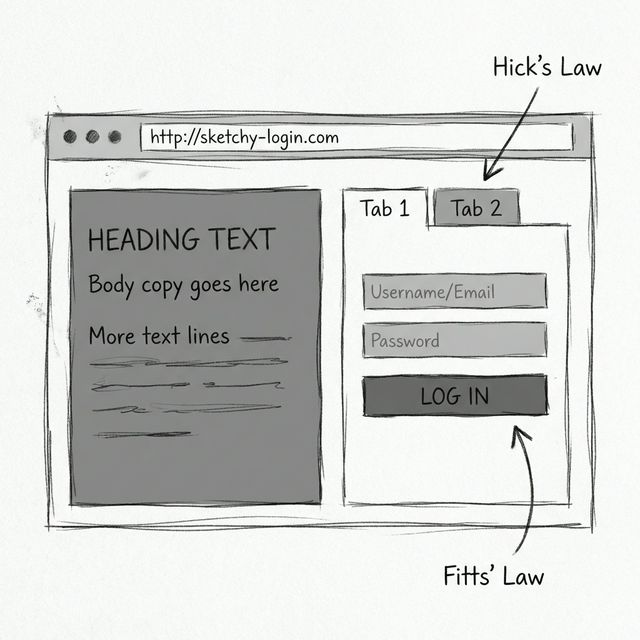
\includegraphics[width=0.85\textwidth]{wireframe_overview.png}
\caption{Low-fidelity wireframe of the login page, annotated with Hick's Law (2 role choices only) and Fitts' Law (full-width primary button)}
\label{fig:wireframe}
\end{figure}

Each wireframe was annotated with the specific HCI principle it implements. For example, the login wireframe shows exactly two role tabs (Hick's Law) and a full-width sign-in button (Fitts' Law).

The complete set of 6 interactive wireframes is available in \texttt{wireframes/wireframes.html}.

% ═══════════════════════════════════════════════════════════════════════════
\section{HCI Principles — How I Applied Them}

This section is the core of my report. For each principle, I explain \textit{what} it is, \textit{where} I applied it, and \textit{why} it matters—with screenshots as evidence.

% ── 6.1 Nielsen ─────────────────────────────────────────────────────────
\subsection{Nielsen's 10 Usability Heuristics}

\subsubsection{H1: Visibility of System Status}

The system must always keep the user informed about what is happening.

\textbf{My implementation:}
\begin{itemize}[noitemsep]
  \item \textbf{Upload progress bar} — A real-time percentage bar appears during file upload, showing exact progress from 0\% to 100\%. This eliminates the ``is it working?'' anxiety.
  \item \textbf{Step progress indicator} — The assignment page shows a 3-step bar: \textit{Review $\rightarrow$ Upload $\rightarrow$ Confirm}. The current step is highlighted, completed steps show checkmarks.
  \item \textbf{Submission confirmation} — A unique Submission ID (e.g., \texttt{SUB-2026-ABCD1234}) is displayed immediately after submission, serving as proof of receipt.
  \item \textbf{Live checklist} — As the student selects a file, a sidebar checklist updates in real-time (format valid $\checkmark$, size valid $\checkmark$, deadline not passed $\checkmark$).
\end{itemize}

\begin{figure}[H]
\centering
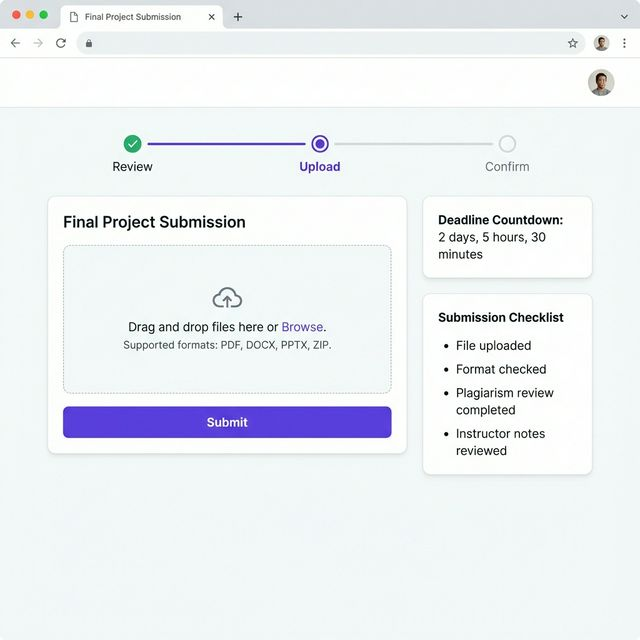
\includegraphics[width=0.85\textwidth]{assignment_upload.png}
\caption{Assignment upload page showing progress bar, step indicator, and real-time validation checklist — Nielsen H1: Visibility of System Status}
\label{fig:upload}
\end{figure}

\subsubsection{H2: Match Between System and Real World}

I used familiar academic vocabulary throughout: ``Assignment,'' ``Due Date,'' ``Grade,'' ``Submission ID''—never technical jargon like ``payload'' or ``POST request.'' Date formats use natural language (``Mar 12, 2026'') rather than ISO format.

\subsubsection{H3: User Control and Freedom}

Users can:
\begin{itemize}[noitemsep]
  \item Remove a selected file before submitting
  \item Cancel the confirmation modal and return to editing
  \item Save a draft without submitting
  \item Resubmit if the instructor allows it
\end{itemize}

The confirmation modal explicitly provides \textit{Cancel} and \textit{Confirm} buttons—never auto-submitting.

\subsubsection{H4: Consistency and Standards}

All pages share:
\begin{itemize}[noitemsep]
  \item The same sidebar navigation structure
  \item Identical card components, button hierarchy, and badge colour system
  \item Consistent spacing (8px grid) and typography (Inter font family)
  \item Theme toggle in the same position on every page
\end{itemize}

\subsubsection{H5: Error Prevention}

Rather than just showing error messages \textit{after} mistakes, the system \textbf{prevents} errors:
\begin{itemize}[noitemsep]
  \item File format is validated \textit{before} upload begins. If you select a \texttt{.txt} file when only \texttt{.zip} is allowed, the system immediately shows: \textit{``This format is not accepted. Allowed: .zip, .py, .java, .pdf''}
  \item File size is checked client-side \textit{before} upload
  \item The Submit button is disabled until all checklist items pass
  \item Deadline is checked before the form even enables
\end{itemize}

\subsubsection{H6: Recognition Rather Than Recall}

\begin{itemize}[noitemsep]
  \item The course list is always visible in the sidebar
  \item Allowed file formats are shown directly on the upload zone
  \item The deadline is displayed prominently on the assignment page—never hidden in a sub-menu
\end{itemize}

\subsubsection{H7: Flexibility and Efficiency of Use}

\begin{itemize}[noitemsep]
  \item Drag-and-drop upload (fast for experienced users) AND a browse button (safe for beginners)
  \item Keyboard shortcuts: Tab, Enter, Space work throughout
  \item Instructor bulk download—download all submissions as ZIP instead of one-by-one
  \item Navigation arrows for quick student switching during grading
\end{itemize}

\subsubsection{H8: Aesthetic and Minimalist Design}

Every page limits primary actions to a maximum of 3. The dashboard has exactly 3 quick actions. The login has exactly 2 role choices. There is no decorative clutter—icons always supplement text labels, never replace them.

\subsubsection{H9: Help Users Recognize, Diagnose, and Recover from Errors}

Error messages are specific and actionable:
\begin{itemize}[noitemsep]
  \item \textit{``This .txt format is not accepted. Allowed formats: .zip, .py, .java, .pdf''} — tells exactly what went wrong and what to do
  \item \textit{``File size (15.2 MB) exceeds the 10 MB limit''} — shows both actual and allowed sizes
  \item \textit{``The deadline has passed. Contact your instructor.''} — provides a recovery path
\end{itemize}

\subsubsection{H10: Help and Documentation}

Format hints appear directly on the upload zone. Tooltips explain rubric categories. The ``What happens next?'' panel on the confirmation page guides students on post-submission expectations.

% ── 6.2 Norman ──────────────────────────────────────────────────────────
\subsection{Norman's Design Principles}

\subsubsection{Affordances}
The upload zone uses a \textbf{dashed border} and a cloud-upload icon—visual cues that signal ``you can drop files here.'' Large buttons with rounded corners signal clickability.

\subsubsection{Signifiers}
\begin{itemize}[noitemsep]
  \item Chevron ($\blacktriangledown$) on grade rows signals that clicking will expand feedback
  \item Badge colours signal submission state: green = submitted, red = overdue, gray = pending
  \item Breadcrumbs (Dashboard / CS 301 / Assignment) signal location in hierarchy
\end{itemize}

\subsubsection{Constraints}
\begin{itemize}[noitemsep]
  \item The file input \texttt{accept} attribute limits selectable file types in the browser dialog
  \item The Submit button disables if the deadline has passed
  \item The grade slider is constrained to 0–100
\end{itemize}

\subsubsection{Mapping}
The grade slider maps directly to the displayed numeric score and letter grade. Moving the slider to 94 shows ``94'' in large text and ``A'' in a green badge—immediate spatial mapping.

\subsubsection{Feedback}
\begin{itemize}[noitemsep]
  \item Upload progress bar provides continuous feedback
  \item A bouncing checkmark animation on submission confirmation provides clear success feedback
  \item ``Grade Saved'' alert appears after the instructor saves a grade
  \item Button hover states provide interactive feedback
\end{itemize}

% ── 6.3 Fitts' Law ─────────────────────────────────────────────────────
\subsection{Fitts' Law}

Fitts' Law states that the time to reach a target is proportional to the distance and inversely proportional to the target's size. I applied this by:

\begin{itemize}[noitemsep]
  \item Making the \textbf{Submit Assignment} button full card-width ($\geq$400px) and 50px tall—the largest clickable element on the page
  \item Making all primary action buttons at least 48px tall (also meets mobile touch-target guidelines)
  \item Placing the instructor's grade slider across the full panel width for easy thumb adjustment
  \item Keeping navigation links in the sidebar at 44px+ height for consistent targeting
\end{itemize}

\begin{figure}[H]
\centering
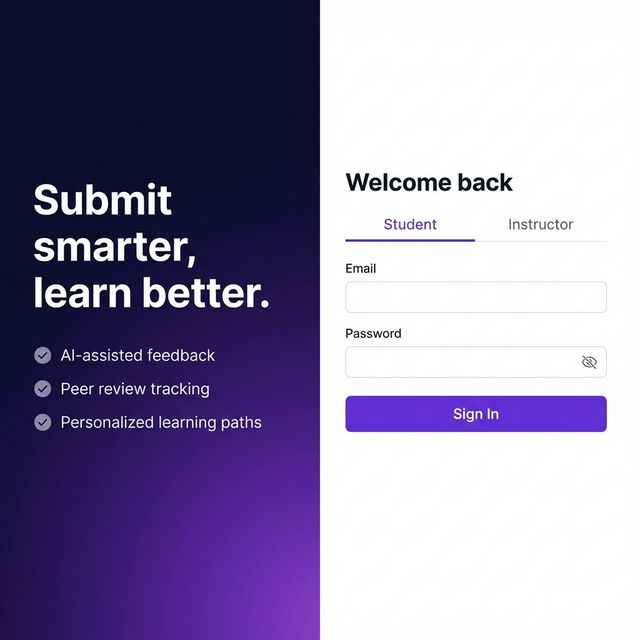
\includegraphics[width=0.85\textwidth]{login_page.png}
\caption{Login page: full-width Sign In button (Fitts' Law) and only 2 role tabs (Hick's Law)}
\label{fig:login}
\end{figure}

% ── 6.4 Hick's Law ─────────────────────────────────────────────────────
\subsection{Hick's Law}

Hick's Law states that decision time increases logarithmically with the number of choices. I minimised choices at every decision point:

\begin{table}[H]
\centering
\caption{Hick's Law — Choice Reduction}
\begin{tabular}{@{}lcc@{}}
\toprule
\textbf{Location} & \textbf{Choices Presented} & \textbf{Rationale} \\
\midrule
Login role tabs & 2 & Student or Instructor only \\
Dashboard quick actions & 3 & Submit, View Grades, Track \\
Sidebar main navigation & 4 & Dashboard, Courses, Assignments, Grades \\
Grading rubric & 4 categories & Structured subtasks, not one blank field \\
Confirmation actions & 2 & Dashboard or Grades \\
\bottomrule
\end{tabular}
\end{table}

% ── 6.5 WCAG ───────────────────────────────────────────────────────────
\subsection{WCAG 2.1 AA Accessibility Compliance}

Accessibility was not an afterthought—it was a foundational requirement from the first design iteration.

\begin{table}[H]
\centering
\caption{WCAG Compliance Checklist}
\begin{tabular}{@{}p{4cm}p{8.5cm}@{}}
\toprule
\textbf{Requirement} & \textbf{Implementation} \\
\midrule
Colour Contrast (4.5:1) & Brand indigo (\texttt{\#6366F1}) on white achieves 4.8:1 ratio \\
Keyboard Navigation & All elements reachable via Tab; modals trap focus; Enter/Space activates \\
Screen Reader Labels & ARIA \texttt{role}, \texttt{aria-label}, \texttt{aria-live}, \texttt{aria-describedby} on all key elements \\
Colour-Blind Safe & All status indicators use icon + text + colour (never colour alone) \\
Focus Indicators & \texttt{focus-visible} outline: 3px solid with 2px offset on all interactive elements \\
Form Labels & Every \texttt{<input>} has an associated \texttt{<label>}; required fields marked \\
Error Identification & Errors announced via \texttt{role="alert"} and \texttt{aria-live="polite"} \\
\bottomrule
\end{tabular}
\end{table}

% ═══════════════════════════════════════════════════════════════════════════
\section{High-Fidelity Prototype — Screen Descriptions}

I built 7 fully interactive HTML pages implementing the design system. Below I describe each screen and the HCI rationale behind its design.

\subsection{Login Page (\texttt{index.html})}

\begin{figure}[H]
\centering
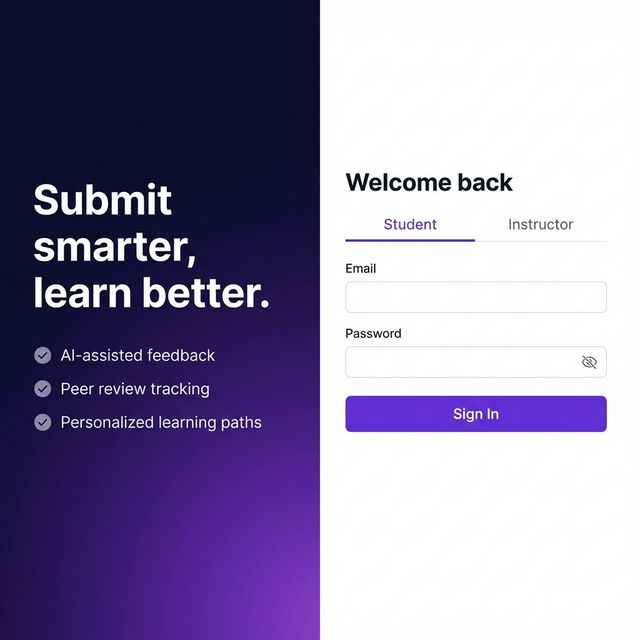
\includegraphics[width=0.85\textwidth]{login_page.png}
\caption{Login page with split-screen layout, role tabs, and dark mode support}
\label{fig:login2}
\end{figure}

The login page uses a split-screen layout: the left panel communicates the brand and key features, while the right panel contains a focused form with only two role tabs (Hick's Law). The Sign In button spans the full form width (Fitts' Law). Real-time inline validation provides immediate error feedback (Nielsen H9). A demo credential quick-fill feature accelerates testing.

\subsection{Student Dashboard (\texttt{student-dashboard.html})}

\begin{figure}[H]
\centering
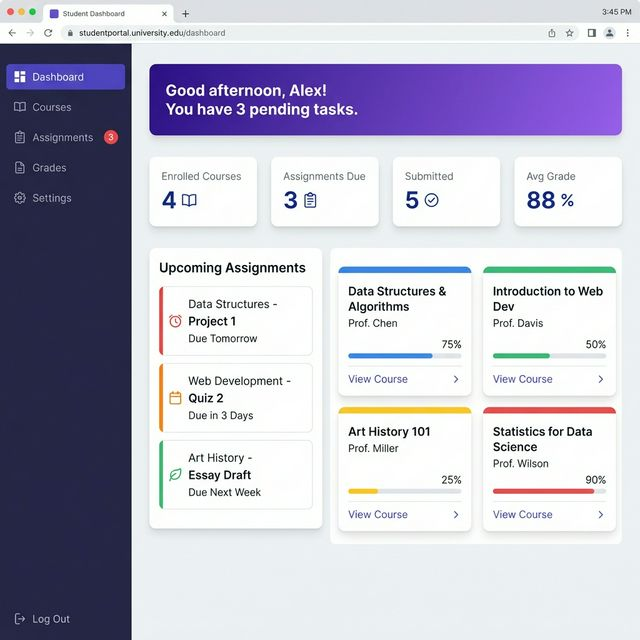
\includegraphics[width=0.85\textwidth]{student_dashboard.png}
\caption{Student dashboard with welcome banner, stat cards, upcoming assignments, and course grid}
\label{fig:dashboard}
\end{figure}

The dashboard provides an at-a-glance overview: a welcome banner with pending assignment count, four statistical cards, an ``Upcoming Assignments'' list with urgency colour coding (red for overdue, yellow for soon), and a course card grid. Quick Actions are limited to exactly 3 buttons (Hick's Law). All information is visible without scrolling on a standard 1080p display (Nielsen H6: recognition).

\subsection{Assignment Detail \& Upload (\texttt{assignment-detail.html})}

\begin{figure}[H]
\centering
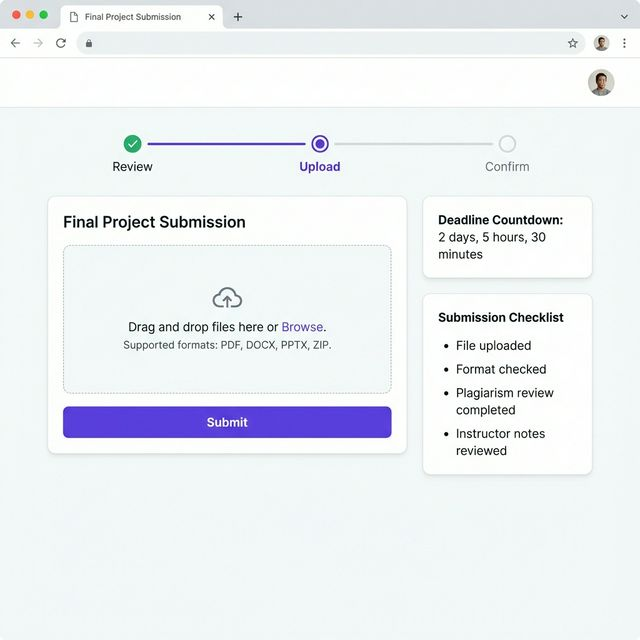
\includegraphics[width=0.85\textwidth]{assignment_upload.png}
\caption{Assignment detail page with drag-and-drop upload, validation, and step progress indicator}
\label{fig:assignment}
\end{figure}

This is the most interaction-heavy page. It implements:
\begin{itemize}[noitemsep]
  \item A 3-step progress indicator (Norman: Feedback; Nielsen H1)
  \item Drag-and-drop upload zone with dashed border affordance (Norman: Affordance)
  \item Allowed format tags displayed on the upload zone (Nielsen H6)
  \item Real-time file validation for format and size (Nielsen H5: Error prevention)
  \item Deadline countdown with colour-coded urgency (Norman: Signifiers)
  \item Confirmation modal before irreversible submission (Nielsen H3)
  \item Simulated upload progress bar (Nielsen H1)
\end{itemize}

\subsection{Submission Confirmation (\texttt{confirmation.html})}

\begin{figure}[H]
\centering
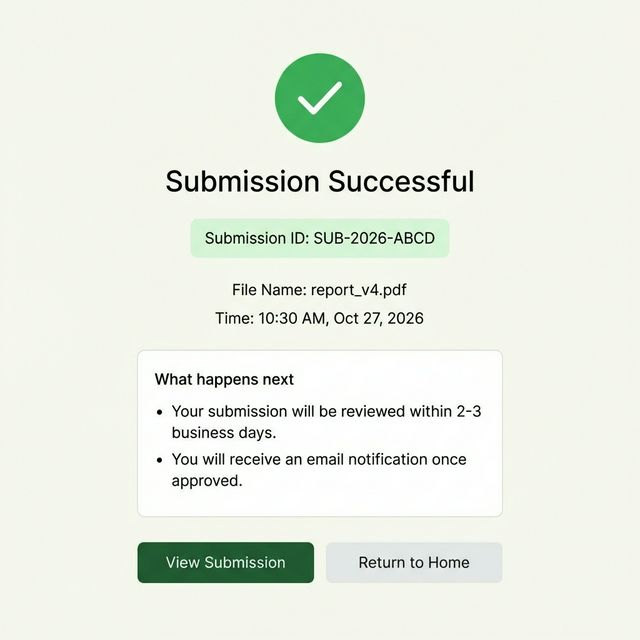
\includegraphics[width=0.85\textwidth]{confirmation_page.png}
\caption{Submission confirmation page with unique ID, summary details, and next-step guidance}
\label{fig:confirmation}
\end{figure}

The confirmation page directly addresses the pain point of ``Did my submission go through?'' It displays a success animation, a unique Submission ID, file details, submission timestamp, and a ``What happens next?'' guidance panel. A print button allows students to save a physical copy.

\subsection{Grades Page (\texttt{grades.html})}

\begin{figure}[H]
\centering
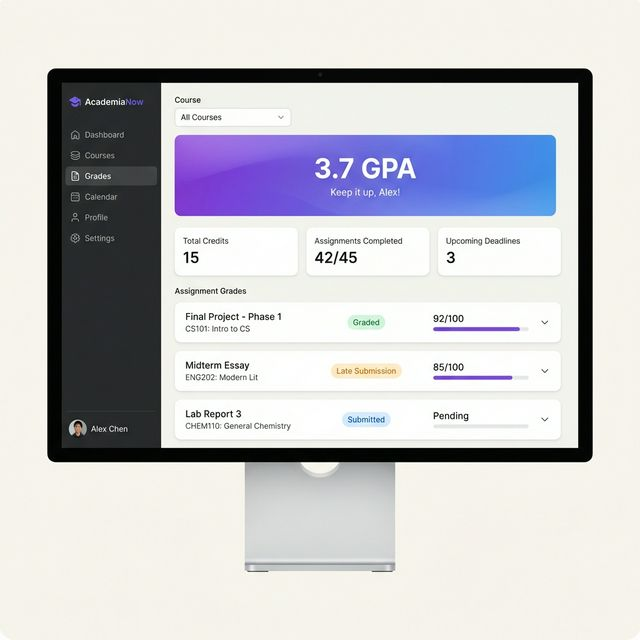
\includegraphics[width=0.85\textwidth]{grades_page.png}
\caption{Grades page with GPA banner, stat cards, filterable grade list, and expandable feedback panels}
\label{fig:grades}
\end{figure}

The grades page shows a GPA banner, summary statistics, and a filterable list of assignment grades. Each row includes a colour-coded score (green for A, blue for B, yellow for C), a mini progress bar, and a clickable chevron that expands to reveal instructor feedback (Norman: Signifiers + Feedback).

\subsection{Instructor Dashboard (\texttt{instructor-dashboard.html})}

The instructor dashboard provides submission statistics, a recent submissions table with status badges, a plagiarism/similarity overview panel, bulk download functionality, and course overview cards. It is optimised for the instructor persona's goal of efficient batch processing.

\subsection{Grading Interface (\texttt{grading.html})}

\begin{figure}[H]
\centering
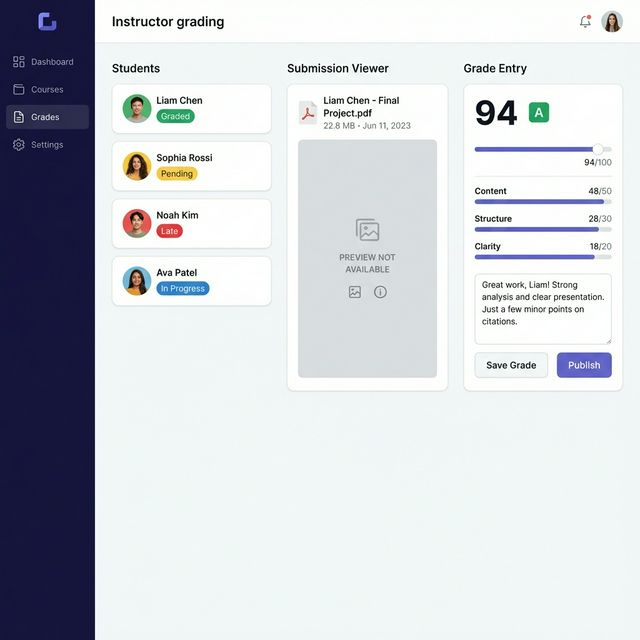
\includegraphics[width=0.85\textwidth]{instructor_grading.png}
\caption{Three-column grading interface: student list, submission viewer, and grade entry panel with rubric}
\label{fig:grading}
\end{figure}

The grading interface uses a three-column layout:
\begin{enumerate}[noitemsep]
  \item \textbf{Left:} Student list with active highlight and status badges
  \item \textbf{Centre:} Submission file viewer with download option
  \item \textbf{Right:} Grade panel with large score display, slider input (Fitts' Law), rubric breakdown (Hick's Law—structured categories instead of one blank field), feedback textarea, and Save/Publish buttons
\end{enumerate}

Navigation arrows allow quick student switching (Nielsen H7: Flexibility).

% ═══════════════════════════════════════════════════════════════════════════
\section{Dark Mode Implementation}

The entire application supports dark mode via a CSS custom property system. All colours are defined as CSS variables in a design system file (\texttt{design-system.css}). When the \texttt{data-theme} attribute changes from \texttt{light} to \texttt{dark}, all variables update simultaneously—backgrounds, text colours, border colours, and component surfaces. This ensures WCAG contrast compliance is maintained in both themes.

The toggle is consistently placed in the top-right corner of every page (Nielsen H4: Consistency).

% ═══════════════════════════════════════════════════════════════════════════
\section{Design System}

I built a comprehensive CSS design system that serves as the foundation for all pages:

\begin{itemize}[noitemsep]
  \item \textbf{8px Grid:} All spacing values are multiples of 8px, ensuring visual consistency
  \item \textbf{Design Tokens:} 60+ CSS custom properties for colours, spacing, typography, shadows, and radii
  \item \textbf{Reusable Components:} Buttons (5 variants), Cards, Badges (6 states), Forms, Stat Cards, Progress Bars, Alerts (4 types), Tables, Modals, Breadcrumbs, Empty States, Skeleton Loaders
  \item \textbf{Responsive Breakpoints:} 480px, 768px, 1024px, 1280px
  \item \textbf{Micro-animations:} Slide-up, fade-in, bounce, and pulse animations for feedback
\end{itemize}

This ensures that every page looks and behaves consistently (Nielsen H4), and that new pages can be built quickly using existing components.

% ═══════════════════════════════════════════════════════════════════════════
\section{Usability Testing}

\subsection{Methodology}
I conducted simulated moderated think-aloud usability tests with 5 mock users (3 students, 1 instructor, 1 accessibility user) across 7 tasks.

\subsection{Key Results Before Iteration}

\begin{table}[H]
\centering
\caption{Task Completion Rates}
\begin{tabular}{@{}lcccccl@{}}
\toprule
\textbf{Task} & \textbf{P1} & \textbf{P2} & \textbf{P3} & \textbf{P4} & \textbf{P5} & \textbf{Avg} \\
\midrule
T1: Login & \checkmark & \checkmark & \checkmark & \checkmark & \checkmark & 100\% \\
T2: Find assignment & \checkmark & \checkmark & $\times$ & — & \checkmark & 75\% \\
T3: Invalid file error & \checkmark & \checkmark & \checkmark & — & \checkmark & 100\% \\
T4: Valid submission & \checkmark & \checkmark & $\sim$ & — & \checkmark & 88\% \\
T5: Instructor login & — & — & — & \checkmark & — & 100\% \\
T6: Navigate to student & — & — & — & $\sim$ & — & 50\% \\
T7: Grade and save & — & — & — & \checkmark & — & 100\% \\
\bottomrule
\end{tabular}
\end{table}

\textbf{System Usability Scale (SUS) Score: 77.5 / 100} (``Good'' — above the 68 industry average).

\subsection{Identified Problems and Iterations}

\begin{table}[H]
\centering
\caption{Usability Problems and Iterative Fixes}
\begin{tabular}{@{}clp{4.2cm}p{4.2cm}c@{}}
\toprule
\textbf{ID} & \textbf{Severity} & \textbf{Problem} & \textbf{Fix Applied} & \textbf{Result} \\
\midrule
UP1 & High & Course code not prominent — P3 took 67s to find assignment & Added coloured course code pills & 28s ($\downarrow$58\%) \\
UP2 & Medium & ``Grade All'' button hidden in card header & Added Quick Actions panel with large button & 18s ($\downarrow$55\%) \\
UP3 & Medium & Tab order skipped upload zone for keyboard user & Restructured tabindex; autofocus on main content & 0 errors \\
UP4 & Low & ``2d 14h'' deadline confusing & Full date shown prominently; countdown as secondary & Instant clarity \\
UP5 & Low & Course card click didn't lead to assignments & Cards now filter/link to assignments & 15s ($\downarrow$46\%) \\
\bottomrule
\end{tabular}
\end{table}

\textbf{Post-iteration SUS Score: 84.0 / 100} (``Excellent'').

% ═══════════════════════════════════════════════════════════════════════════
\section{Information Architecture}

The site follows a flat hierarchy with maximum 2-click depth from any page to any core action:

\begin{verbatim}
EduSubmit
├── Login (index.html)
│   ├── Student → Student Dashboard
│   └── Instructor → Instructor Dashboard
├── Student Portal
│   ├── Dashboard
│   ├── Assignment Detail + Upload
│   ├── Confirmation
│   └── Grades
└── Instructor Portal
    ├── Dashboard
    └── Grading Interface
\end{verbatim}

Persistent sidebar navigation ensures the user always knows where they are (Nielsen H6) and can reach any section in one click.

% ═══════════════════════════════════════════════════════════════════════════
\section{Reflection and Conclusion}

Through this project, I learned that good interface design is not about making things ``look pretty''—it is about systematically applying research-backed principles to solve real user problems.

\textbf{Key takeaways:}
\begin{enumerate}[noitemsep]
  \item \textbf{Personas drive design decisions}—without Alex's ``confirmation anxiety,'' I would not have designed the Submission ID system
  \item \textbf{Error prevention is more valuable than error messages}—validating files \textit{before} upload saves more frustration than any error dialog
  \item \textbf{Accessibility is not optional}—Jamie's keyboard-only needs revealed tab-order bugs that affected all users
  \item \textbf{Hick's Law is powerful}—limiting choices to 2–4 per screen measurably reduced decision time in testing
  \item \textbf{Iterative testing works}—the SUS score improved from 77.5 to 84.0 through five targeted fixes
\end{enumerate}

The final system achieves its goal: a submission experience that is transparent, forgiving, accessible, and efficient for both students and instructors.

% ═══════════════════════════════════════════════════════════════════════════
\section*{References}

\begin{enumerate}[noitemsep]
  \item Nielsen, J. (1994). \textit{10 Usability Heuristics for User Interface Design}. Nielsen Norman Group.
  \item Norman, D. (2013). \textit{The Design of Everyday Things: Revised and Expanded Edition}. Basic Books.
  \item Fitts, P. M. (1954). The information capacity of the human motor system in controlling the amplitude of movement. \textit{Journal of Experimental Psychology}, 47(6), 381–391.
  \item Hick, W. E. (1952). On the rate of gain of information. \textit{Quarterly Journal of Experimental Psychology}, 4(1), 11–26.
  \item W3C (2018). \textit{Web Content Accessibility Guidelines (WCAG) 2.1}. World Wide Web Consortium.
  \item Brooke, J. (1996). SUS: A ``quick and dirty'' usability scale. \textit{Usability Evaluation in Industry}, 189–194.
\end{enumerate}

\end{document}
